\graphicspath{{Chapter2/Figs/}}

\section{Multi-Omics Factor Analysis: a framework for unsupervised integration of multi-omics data sets}
% In the first section of this chapter, we will describe XXX

The work described in this chapter results from a collaboration with the Multi-omics and statistical computing group lead by Wolfgang Huber at the EMBL (Heidelberg, Germany). It has been peer-reviewed and published in Argelaguet \& Velten et al \cite{Argelaguet2018}.\\

The method was conceived by Florian Buettner, Oliver Stegle and me. I performed most of the mathematical derivations and implementation, but with significant contributions from Damien Arnol and Britta Velten. The single-cell application was led by me whereas the CLL data application was led by Britta Velten, but with joint contributions in either cases. Florian Buettner, Wolfgang Huber and Oliver Stegle supervised the project.\\
The article was jointly written by Britta Velten, Florian Buettner, Wolfgang Huber, Oliver Stegle and me.


\subsection{Model description}
MOFA is a multi-view generalisation of traditional Factor Analysis to $M$ input matrices (or views) $\bfY^m \in \R^{N \times D_m}$ based on the framework of Group Factor Analysis (discussed in Section X).\\
The input data consists on $M$ views with non-overlapping features that often represent different assays. However, there is flexibility in the definition of views and they can be tailored to address different hypothesis.\\
%For example, if one has DNA methylation data, one could define as a single view the matrix with all genome-wide measurements, but one could also split this matrix into different views, either by chromosome or by genomic context (i.e. promoters, enhancers, etc.).\\
Formally, the input data is factorised as:
\begin{equation}
	\mathbf{Y}^m = \mathbf{Z}\mathbf{W}^{mT} + \bepsilon^m
\end{equation}
where $\bfZ \in \R^{N \times K}$ is a matrix that contains the factor values and $\bfW^m \in \R^{D_m \times K}$ are $M$ matrices that contain the loadings that relate the high-dimensional space to the low-dimensional latent representation. Finally, $\bepsilon^m \in \R^{D_m}$ captures the residuals, or the noise, which is assumed to be normally distributed and heteroskedastic:
\begin{equation}
	p(\epsilon^m_d) = \Ndist{\epsilon^m_d}{0,1/\tau_d^m}
\end{equation}
Non-gaussian noise models can also be defined and is discussed in Section XX. Unless otherwise stated, we will always assume Gaussian noise.\\
Altogether, this results in the following likelihood:
\begin{equation}
	p(\bfY|\bfW,\bfZ,\bTau) = \prod_{m=1}^{M} \prod_{d=1}^{D_m} \prod_{n=1}^{N} \Ndist{y_{nd}^m}{\bfz_{n}^T\bfw_{d}^{m},1/\tau_d^m}
	% p(y_{nd}^m) = \Ndist{y_{nd}^m}{\bfz_{n,:}\bfw_{d,:}^{mT},1/\tau_d^m},
\end{equation}

\subsubsection{Interpretation of the factors}
Each factor ordinates cells along a one-dimensional axis centered at zero. Samples with different signs indicate opposite phenotypes, with higher absolute value indicating a stronger effect. For example, if the $k$-th factor captures the variability associated with cell cycle, we could expect cells in the Mitosis state to be at one end of the factor (irrespective of the sign, only the relative positioning being of importance). In contrast, cells in G1 phase are expected to be at the other end of the factor. Cells with intermediate phenotype, or with no clear phenotype (i.e. no cell cycle genes profiled), are expected to be located around zero, as specified by the prior distribution.

\subsubsection{Interpretation of the loadings}
The loadings provide a score for each gene on each factor, and are interpreted in a similar way as the factors. Genes with no association with the factor are expected to have values close to zero, as specified by the prior. In contrast, genes with strong association with the factor are expected to have large absolute values. The sign of the loading indicates the direction of the effect: a positive loading indicates that the feature is more active in the cells with positive factor values, and viceversa. \\
Following the cell cycle example from above, we expect genes that are upregulated in the M phase to have large positive loadings, whereas genes that are downregulated in the M phase (or, equivalently, upregulated in the G1 phase) are expected to have large negative loadings.\\

% The following figure shows a real-case example of a Factor capturing the cell cycle effect, with the corresponding loadings:

% \begin{figure}[H]
% 	\begin{center}
% 		\includegraphics[width=1.0\textwidth]{figures/cell_cycle}
% 		\caption{Example of a factor (Factor 2) that captures the cell cycle phenotype. Left shows a scatterplot of Factor 1 and Factor 2, where each dot is a single cell. The cells are colored by the infered lineage and they are shaped by the infered cell cycle phase. Right shows the RNA expression loadings for Factor 5. Each dot represents a gene.  }
% 		\label{fig:cell_cycle}
% 	\end{center}
% \end{figure}


\subsubsection{Interpretation of the noise}
The use of a probabilistic framework allows the model to explicitly disentangle the signal (i.e. the explained variance) from the noise (i.e. unexplained variance). Large values of $\tau_d^m$ indicate high certainity on the observations for the feature $d$ in view $m$, as predicted by the latent variables. In contrast, small values of $\tau_d^m$ are indicative of low predictive power by the latent variables.

\subsubsection{Missing values}
The probabilistic formalism naturally accounts for incomplete data matrices, as missing observations do not intervene in the likelihood.\\
In practice, we implement this using memory-efficient binary masks $\mathcal{O}^m \in \mathbb{R}^{N\times D_m}$ for each view $m$, such that $\mathcal{O}_{n,d} = 1$ when feature $d$ is observed for sample $n$, 0 otherwise. 

\subsubsection{Prior distributions for the factors and the loadings}
The key determinant of the model is the regularization used on the prior distributions of the factors and the weights.\\
For the factors, we follow common practice \cite{XX} and define an isotropic Gaussian prior:
\begin{equation}
	p(z_{nk}) = \Ndist{z_{nk}}{0,1}
\end{equation}
For the weights we encode two levels of sparsity, a (1) view- and factor-wise sparsity and (2) an individual feature-wise sparsity. The aim of the factor- and view-wise sparsity is to disentangle the activity of factors to the different views, such that the weight vector $\bfw_{:,k}^m$ is shrunk to zero if the factor $k$ does not explain any variation in view $m$. \\
In addition, we place a second layer of sparsity which encourages inactive weights on each individual feature. Mathematically, we express this as a combination of an Automatic Relevance Determination (ARD) prior \cite{Mackay1996} for the view- and factor-wise sparsity and a spike-and-slab prior \cite{Mitchell1988} for the feature-wise sparsity:
% \begin{equation*}
% 	p(w_{dk}^{m}) = (1-\theta_{k}^{m}) \mathds{1}_0(w_{dk}^{m}) + \theta_{k}^{m} \Ndist{w_{dk}^{m}}{0, 1 / \alpha_{k}^{m}}
% \end{equation*}
However, this formulation of the spike-and-slab prior contains a Dirac delta function, which makes the inference procedure troublesome. To solve this we introduce a re-parametrization of the weights $w$ as a product of a Gaussian random variable $\hat{w}$ and a Bernoulli random variable $s$, \cite{Titsias2011} resulting in the following prior:
% \begin{equation}
% 	p(\hat{w}_{dk}^m,s_{dk}^m) &= \Ndist{\hat{w}_{dk}^m}{0, 1/\alpha_k^m}  \text{Ber}(s_{dk}^m \,|\,\theta_k^m)
% \end{equation}
In this formulation $\alpha_k^m$ controls the activity of factor $k$ in view $m$ and $\theta_k^m$ controls the corresponding fraction of active loadings (i.e. the sparsity levels).\\

Finally, we define conjugate priors for $\theta$ and $\alpha$:
\begin{align}
	p(\theta_k^m) &= \Bdist{\theta_k^m}{a_0^\theta,b_0^\theta}\\
	p(\alpha_k^m) &= \Gdist{\alpha_k^m}{a_0^\alpha, b_0^\alpha},
\end{align}
with hyper-parameters $a_0^\theta,b_0^\theta =1$ and $a_0^\alpha, b_0^\alpha=1e^{-3}$ to get uninformative priors.\\
Posterior values of $\theta_k^m$ close to $0$ implies that most of the weights of factor $k$ in view $m$ are shrinked to $0$ (sparse factor). In contrast, a value of $\theta_k^m$ close to $1$ implies that most of the weights are non-zero (non-sparse factor). A small value of $\alpha_k^m$ implies that factor $k$ is active in view $m$. In contrast, a large value of $\alpha_k^m$ implies that factor $k$ is inactive in view $m$.\\

All together, the joint probability density function of the model is given by
\begin{align}
	\begin{split}
	p(\bfY,\hat{\bfW},\bfS,\bfZ,\btheta, \balpha, \btau)  = &\prod_{m=1}^{M} \prod_{n=1}^{N} \prod_{d=1}^{D_m} \Ndist{y_{nd}^m}{\sum_{k=1}^{K} s_{dk}^m \hat{w}_{dk}^m z_{nk},1/\tau_d} \\
	& \prod_{m=1}^{M}\prod_{d=1}^{D_m} \prod_{k=1}^{K} \Ndist{\hat{w}_{dk}^m}{0,1/\alpha_k^m} \text{Ber}(s_{d,k}^m|\theta_k^m) \\
	& \prod_{n=1}^{N} \prod_{k=1}^{K} \Ndist{z_{nk}}{0,1} \\
	& \prod_{m=1}^{M} \prod_{k=1}^{K} \Bdist{\theta_k^m}{a_0^\theta,b_0^\theta}\\
	& \prod_{m=1}^{M} \prod_{k=1}^{K} \Gdist{\alpha_k^m}{a_0^\alpha, b_0^\alpha}\\
	& \prod_{m=1}^{M} \prod_{d=1}^{D_m} \Gdist{\tau_d^m}{a_0^\tau,b_0^\tau}.
	\label{likelihood}
	\end{split}
\end{align}
and the corresponding graphical model is shown in \Cref{fig:MOFA_graphical_model}. This completes the definition of the MOFA model.

\subsection{Downstream analysis}

Once trained, the MOFA model can be queried for a set of downstream analysis:
\begin{itemize}
	\item \textbf{Variance decomposition}: calculate the variance explained ($R^2$) by each factor in each view. 
	\item \textbf{Ordination of the samples in the latent space}: scatterplots or beeswarm plots of factors, colored or shaped by sample covariates can reveal the main drivers of sample heterogeneity.
	\item \textbf{Inspection of loadings}: the weights (or loadings) can be interpreted as an activity score for each gene on each factor. Hence, inspecting the top loadings reveals the genes (or other genomic features) that underlie each factor.
	\item \textbf{Imputation}: MOFA generates a condensed and denoised low-dimensional representation of the data without missing values. As discussed in Section X, the data can be reconstructed from the latent space by a simple matrix multiplication: $\hat{\bfY} = \bfZ \bfW^T$. 
	\item \textbf{Feature set enrichment analysis}: when a factor is difficult to characterise based only on the inspection of the top loadings, one can compute a statistical test for enrichment of biological pathways using predefined gene-set annotations. The statistical tests that we implemented are outlined in Section X.
\end{itemize}

The downstream functionalities implemented in MOFA are highlighted in \Cref{fig:MOFA}.

\begin{figure}[H]
	\begin{center}
		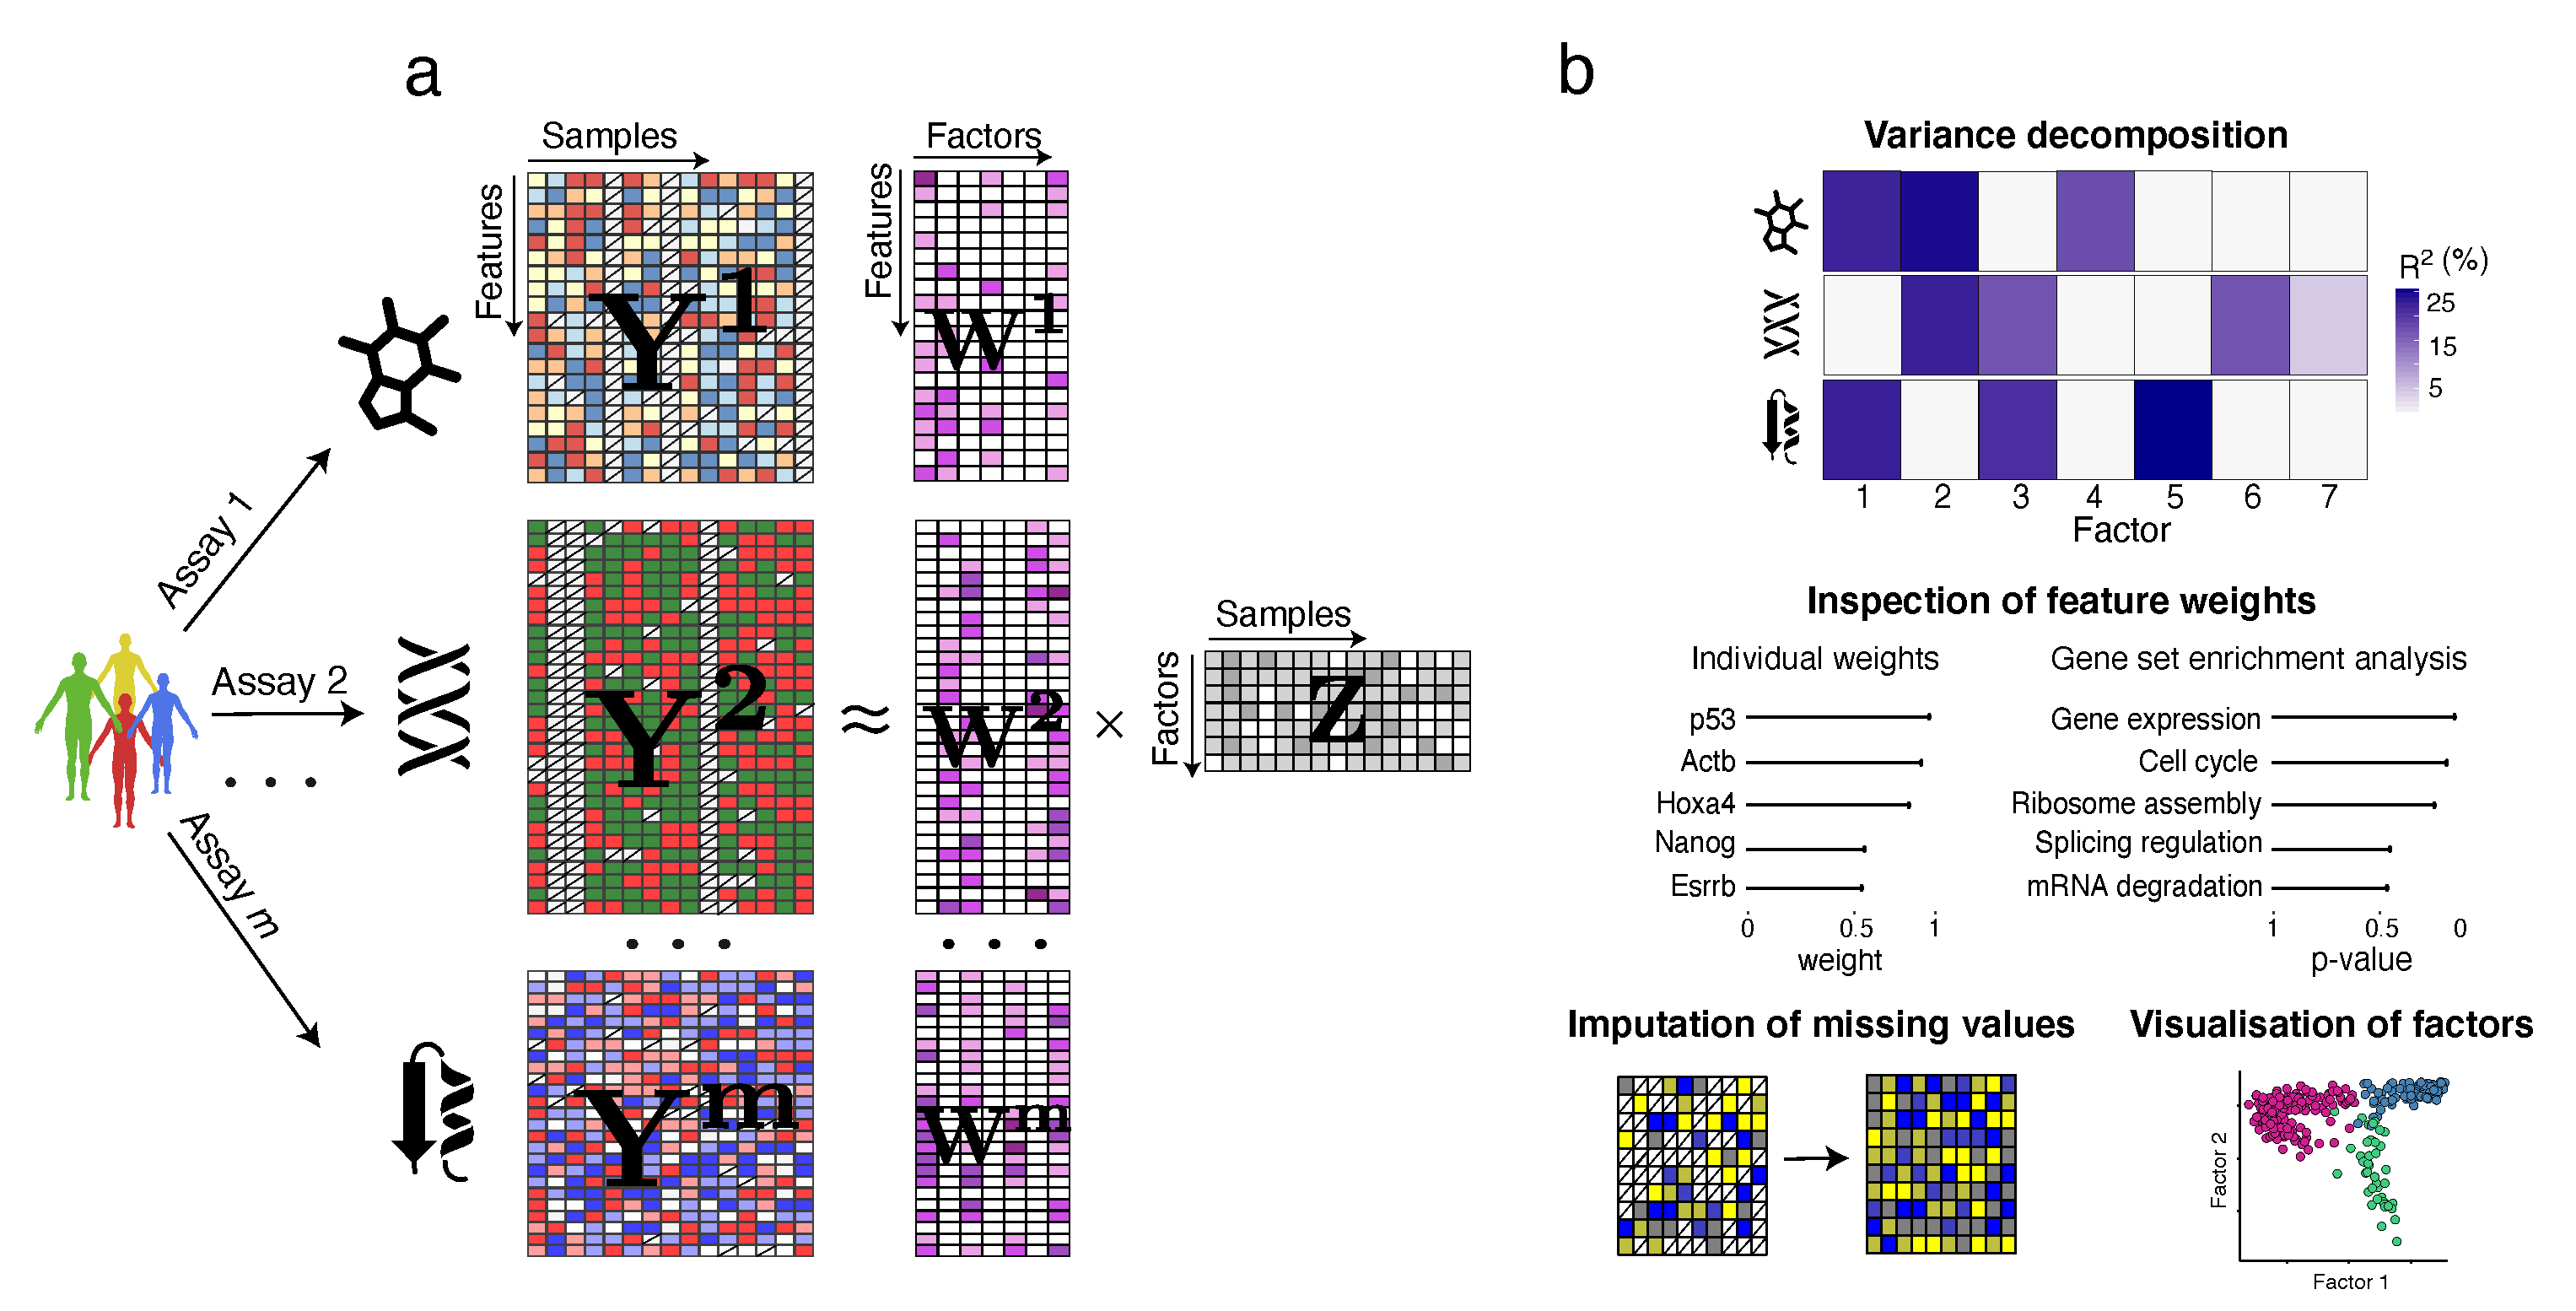
\includegraphics[width=1.0\textwidth]{MOFA}
		\caption{MOFA overview. The model takes $M$ data matrices as input ($\bfY^1, \cdots, \bfY^M$), one or more from each data modality, with co-occurrent samples but features that are not necessarily related and can differ in numbers. MOFA decomposes these matrices into a matrix of factors ($\bfZ$) and $M$ weight matrices, one for each data modality ($\bfW^1, \cdots, \bfW^M$). White cells in the weight matrices correspond to zeros, i.e. inactive features, whereas the cross symbol in the data matrices denotes missing values. The fitted MOFA model can be queried for different downstream analyses, including a variance decomposition to assess the proportion of variance explained by each factor in each data modality.}
		\label{fig:MOFA}
	\end{center}
\end{figure}

\begin{figure}[H]
	\centering
	\section{Multi-Omics Factor Analysis}

###
TO-DO:
- ADD AND DESCIRBE ELBO CURVE, CONVERGENCE		
##


In the first section of this chapter, we will describe XXX

The work discussed in this chapter results from a collaboration with the Multi-omics and statistical computing group lead by Wolfgang Huber (EMBL, Heidelberg, Germany). It has been peer-reviewed and published in Argelaguet \& Belten et al \cite{Clark2018}.\\

The method was conceived by Florian Buettner, Oliver Stegle and me. I performed most of the mathematical derivations and implementation, but with significant contributions from Damien Arnol and Britta Velten. The single-cell application was led by me whereas the CLL data application was mostly led by Britta Velten, but with joint contributions in either cases. Florian Buettner, Wolfgang Huber and Oliver Stegle supervised the project.\\
The article was jointly written by Britta Velten, Florian Buettner, Wolfgang Huber, Oliver Stegle and me.


\subsection{Model description}

MOFA is a multi-view generalisation of traditional Factor Analysis to $M$ input matrices (or views) $\bfY^m \in \R^{N \times D_m}$. Each view consists of non-overlapping features that often represent different assays. However, there is flexibility in the definition of views to address different hypothesis. For example, if one has DNA methylation data, one could define as a single view the matrix with all genome-wide measurements, but one could also split this matrix into different views, either by chromosome or by genomic context (i.e. promoters, enhancers, etc.).\\
Formally, in MOFA, the input data is factorised as:
\begin{equation}
	\mathbf{Y}^m = \mathbf{Z}\mathbf{W}^{mT} + \bepsilon^m,
\end{equation}
where  $\bfZ \in \R^{N \times K}$ is a matrix that contains the factor values and $\bfW^m \in \R^{D_m \times K}$ are $M$ matrices that contain the loadings that relate the high-dimensional space to the low-dimensional latent representation. Finally, $\bepsilon^m \in \R^{D_m}$ captures the residuals, or the noise, which is assumed to be normally distributed and heteroskedastic:
\begin{equation}
	p(\epsilon^m_d) = \Ndist{\epsilon^m_d}{0,1/\tau_d^m}.
\end{equation}
Non-gaussian noise models are available with the same inference framework developed in \cite{Argelaguet2018,Seeger2012,Jaakkola2000}. Unless otherwise stated, we will always assume Gaussian noise.\\
Altogether, this results in the following likelihood:
\begin{equation}
	p(\bfY|\bfW,\bfZ,\bTau) = \prod_{m=1}^{M} \prod_{d=1}^{D_m} \prod_{n=1}^{N} \Ndist{y_{nd}^m}{\bfz_{n}^T\bfw_{d}^{m},1/\tau_d^m},
	% p(y_{nd}^m) = \Ndist{y_{nd}^m}{\bfz_{n,:}\bfw_{d,:}^{mT},1/\tau_d^m},
\end{equation}

\subsubsection{Interpretation of the factors}
Each factor ordinates cells along a one-dimensional axis centered at zero. Samples with different signs indicate opposite phenotypes, with higher absolute value indicating a stronger phenotype. For example, if the $k$-th factor captures the variability associated with cell cycle, we could expect cells in Mitosis to be at one end of the factor (irrespective of the sign, only the relative positioning being of importance). In contrast, cells in G1 phase are expected to be at the other end of the factor. Cells with intermediate phenotype, or with no clear phenotype (i.e. no cell cycle genes profiled), are expected to be located around zero.

\subsubsection{Interpretation of the loadings}
The loadings provide a score for each gene on each factor, and are interpreted in a similar way as the factors. Genes with no association with the factor are expected to have values close to zero, whereas genes with strong association with the factor are expected to have large absolute values. The sign of the loading indicates the direction of the effect: a positive loading indicates that the feature is more active in the cells with positive factor values, and viceversa. \\
Following the cell cycle example from above, we expect genes that are upregulated in the M phase to have large positive loadings, whereas genes that are downregulated in the M phase (or, equivalently, upregulated in the G1 phase) are expected to have large negative loadings.\\

The following figure shows a real-case example of a Factor capturing the cell cycle effect, with the corresponding loadings:

\begin{figure}[H]
	\begin{center}
		\includegraphics[width=1.0\textwidth]{figures/cell_cycle}
		\caption{Example of a factor (Factor 2) that captures the cell cycle phenotype. Left shows a scatterplot of Factor 1 and Factor 2, where each dot is a single cell. The cells are colored by the infered lineage and they are shaped by the infered cell cycle phase. Right shows the RNA expression loadings for Factor 5. Each dot represents a gene.  }
		\label{fig:cell_cycle}
	\end{center}
\end{figure}


\subsubsection{Interpretation of the noise}
The use of a probabilistic framework allows the model to explicitly disentangle the signal, or the explained variance, and the noise or the unexplained variance.
Large values of $\tau_d^m$ indicate high certainity on the observations for the feature $d$ in view $m$, as predicted by the latent variables. In contrast, small values of $\tau_d^m$ are indicative of low predictive power by the latent variables.

\section{Missing values}

(COPIED FROM DAMIEN) Nothing in the Factor Analysis formalism requires the completeness of the data matrices, meaning that these models naturally handle missing values. In a vectorised implementation however, care needs to be taken, so that we keep track of the indices of non-observed data in matrix operations, and remove their contribution to the variational updates and Evidence Lower Bound terms. Biofam encodes the position of the missing values in memory efficient boolean masks, which are built based on the presence of invalid values such as NA in the input matrices, and propagates this information to all update operations.

(COPIED FROM APPENDIX) The model naturally accounts for missing values and no prior imputation is required. Non-observed data points do not intervene in the likelihood and are ignored in the update equations. In practice, we use a binary mask $\mathcal{O}^m \in \mathbb{R}^{N\times D_m}$ for each view $m$, such that $\mathcal{O}_{n,d} = 1$ when feature $d$ is observed for sample $n$, 0 otherwise.

\subsubsection{Prior distributions for the factors and the loadings}
The key determinant of the model is the regularization used on the prior distributions of the factors and the weights. In the first version of MOFA we defined a standard Gaussian prior on the factors:
\begin{equation}
	p(z_{nk}) = \Ndist{z_{nk}}{0,1}
\end{equation}
Effectively this assumes independent and non-sparse samples, a reasonable assumption in datasets with small number of samples and with low amounts of noise, as in bulk studies. \\
In contrast, the weights are assumed to be sparse, the rationality being that the number of features is very large and that real biological factors are driven by potentially small gene regulatory networks \cite{Gao2013}. To achieve this, MOFA encodes two levels of sparsity: (1) a view- and factor-wise sparsity and (2) an individual feature-wise sparsity. The aim of the factor- and view-wise sparsity is to identify which factors are active in which views, such that the weight vector $\bfw_{:,k}^m$ is shrunk to zero if the factor $k$ does not explain any variation in view $m$. \\

In addition, we place a second layer of sparsity which encourages inactive weights on each individual feature. Mathematically, we express this as a combination of an Automatic Relevance Determination (ARD) prior \cite{Mackay1996} for the view- and factor-wise sparsity and a spike-and-slab prior \cite{Mitchell1988} for the feature-wise sparsity:
\begin{equation}
	p(w_{dk}^{m}) = (1-\theta) \mathds{1}_0(w_{dk}^{m}) + \theta \mathcal{N} (w_{dk}^{m} \,|\, 0, 1/\alpha_k^m)
\end{equation}
However, the spike-and-slab prior contains a Dirac delta function, which makes the inference procedure troublesome. To solve this we introduce a re-parametrization of the weights $w$ as a product of a Gaussian random variable $\hat{w}$ and a Bernoulli random variable $s$, \cite{Titsias2011} resulting in the following prior for every single weight $w_{dk}$:
\begin{align}
	p(\hat{w}_{dk}^m,s_{dk}^m) &= \mathcal{N} (\hat{w}_{dk}^m \,|\, 0, 1/\alpha_k^m)\, \text{Ber}(s_{dk}^m \,|\,\theta_k^m)
\end{align}
In this formulation $\alpha_k^m$ controls the strength of factor $k$ in view $m$ and $\theta_k^m$ controls the fraction of non-zero (active) loadings (i.e. the sparsity levels) of factor $k$ in view $m$. Finally, we allow the model to learn the levels of sparsity and introduce the following priors for $\theta$ and $\alpha$:
\begin{align}
	p(\theta_k^m) &= \Bdist{\theta_k^m}{a_0^\theta,b_0^\theta}\\
	p(\alpha_k^m) &= \Gdist{\alpha_k^m}{a_0^\alpha, b_0^\alpha},
\end{align}
with hyper-parameters $a_0^\theta,b_0^\theta =1$ and $a_0^\alpha, b_0^\alpha=1e^{-3}$ to get uninformative priors. Posterior values of $\theta_k^m$ close to $0$ implies that most of the weights of factor $k$ in view $m$ are shrinked to $0$ (sparse factor). In contrast, a value of $\theta_k^m$ close to $1$ implies that most of the weights are non-zero (non-sparse factor). A small value of $\alpha_k^m$ implies that factor $k$ is active in view $m$. In contrast, a large value of $\alpha_k^m$ implies that factor $k$ is inactive in view $m$.\\
This completes the definition of the original model, which is depicted in the following figure:

\begin{figure}[H]
	\begin{center}
		\includegraphics[width=1.0\textwidth]{figures/mofa1}
		\caption{MOFA 1.0 overview. The model takes $M$ data matrices as input ($\bfY^1, \cdots, \bfY^M$), one or more from each data modality, with co-occurrent samples but features that are not necessarily related and can differ in numbers. MOFA decomposes these matrices into a matrix of factors ($\bfZ$) and $M$ weight matrices, one for each data modality ($\bfW^1, \cdots, \bfW^M$). White cells in the weight matrices correspond to zeros, i.e. inactive features, whereas the cross symbol in the data matrices denotes missing values. The fitted MOFA model can be queried for different downstream analyses, including a variance decomposition to assess the proportion of variance explained by each factor in each data modality.}
		\label{fig:MOFA1}
	\end{center}
\end{figure}

\subsection{Modelling and inference with non-Gaussian data} \label{section:non_gaussian}
To implement efficient variational inference in conjunction with a non-Gaussian likelihood we adapt prior work from \cite{seeger} using local variational bounds. The key idea is to dynamically approximate non-Gaussian data by Gaussian pseudo-data based on a second-order Taylor expansion.  To make the approximation justifiable we need to introduce variational parameters that are adjusted alongside the updates to improve the fit.	\\
Denoting the parameters in the MOFA model as $\bfX= (\bfZ,\bfW,\balpha,\btau,\btheta)$, recall that the variational framework approximates the posterior $p(\bfX | \bfY )$ with a distribution $q(\bfX)$, which is indirectly optimised by optimising a lower bound of the log model evidence. The resulting optimization problem can be re-written from \Cref{VBintro} as
\begin{equation*}
\min_{q(\bfX)} -\Lagr(\bfX) =  \min_{q(\bfX)} \E_q \big[ -\log p(\bfY|\bfX) \big] + \KL[q(\bfX)||p(\bfX)].
\end{equation*}


Expanding the MOFA model to non-Gaussian likelihoods we now assume a general likelihood of the form $p(\bfY|\bfX)=p(\bfY|\bfC)$ with $\bfC = \bfZ\bfW^{T}$, that can write as

\begin{equation*}
-\log p(\bfY|\bfX) = \sum_{n=1}^{N} \sum_{d=1}^{D} f_{nd} (c_{nd})
\end{equation*}
with $f_{nd}(c_{nd}) = -\log p(y_{nd}|c_{nd})$. We dropped the view index $m$ to keep notation uncluttered.\\
Extending \cite{seeger} to our heteroscedastic noise model, we require $f_{nd}(c_{nd})$ to be twice differentiable and bounded by $\kappa_d$, such that $f_{nd}''(c_{nd}) \leq \kappa_d \,\forall n,d$. This holds true in many important models as for example the Bernoulli and Poisson case. Under this assumption a lower bound on the log likelihood can be constructed using Taylor expansion,
\begin{equation*}
f_{nd}(c_{nd}) \leq \frac{\kappa_d}{2} (c_{nd} - \zeta_{nd})^2 + f'(\zeta_{nd})(c_{nd} - \zeta_{nd}) + f_{nd}(\zeta_{nd}) := q_{nd}(c_{nd},\zeta_{nd}),
\end{equation*}
where $\bZeta =  \zeta_{nd} $ are additional variational parameters that determine the location of the Taylor expansion and have to be optimised to make the lower bound as tight as possible. Plugging the bounds into above optimization problem, we obtain:
\begin{equation*}
\min_{q(\bfX),\bZeta} \quad \sum_{d=1}^{D}\sum_{n=1}^{N} \E_q [ q_{nd}(c_{nd},\zeta_{nd})] + \KL[q(\bfX)||p(\bfX)]
\end{equation*}
The algorithm propsed in \cite{seeger} then alternates between updates of $\bZeta$ and $\mathrm{q}(\bTheta)$. The update for $\bZeta$ is given by
\begin{equation*}
\zeta \leftarrow \E[\bfW]\E[\bfZ]^{T}
\end{equation*}
where the expctations are taken with respect to the corresponding $q$ distributions.\\
% In order to find the updates for $q(\bTheta)$ we bring the taylor approximation of $q(f_{nd})$ in q audratic form:
% \begin{equation*}
% q(f_{nd},\zeta_{nd}) \propto \frac{\kappa_d}{2}(f_{nd} - (zeta_{nd} - g(\zeta_{nd})/\kappa_d))^2
% \end{equation*}
% and note that this is proportional to the log of a Gaussian distribution $-log \Normal (\hat{y}_{nd}|f_{ng},\frac{1}{ng})$ where $\hat{y}_{nd} = zeta_{nd} - g'(\zeta_{nd})/\kappa_d$ is defined as a pseudodata based on the zero-inflated observations.
% Consequently, for fixed $\zeta_{nd}$, the updates of the variational distributions $Q(X)$ and $Q(W)$ are equivalent to the ones derived in X, but with pseudodata $\hat{Y}$ and precision $\kappa_g$
On the other hand, the updates for $q(\bfX)$ can be shown to be identical to the variational Bayesian updates with a conjugate Gaussian likelihood when replacing the observed data $\bfY$ by a pseudo-data $\hat{\bfY}$ and the precisions $\tau_{nd}$ (which were treated as random variables) by the constant terms $\kappa_d$ introduced above.\\
The pseudodata is given by
\begin{equation*}
\hat{y}_{nd} = \zeta_{nd} - f'(\zeta_{nd})/\kappa_d.
\end{equation*}
Depending on the log likelihoods $f(\cdot)$ different $\kappa_d$ are used resulting in different pseudo-data updates. Two special cases implemented in MOFA are the Poisson and Bernoulli likelihood described in the following.

\subsubsection*{Bernoulli likelihood for binary data}
When the observations are binary, $y \in \{0,1\}$, they can be modelled using a Bernoulli likelihood:
%\begin{equation*}
%p(y|c) = \frac{e^{yc}}{1+e^c}
%\end{equation*}
%The second derivative of the log likelihood is bounded by:
%\begin{equation*}
%f''(c) = \sigma(c)\sigma(-c) \leq 1/4 := \kappa
%\end{equation*}
%where $\sigma$ is the sigmoid function $f(c) = 1/(1+e^{-c})$.\\
%The pseudodata updates are given by
%\begin{equation*}
%\hat{y}_{nd} = \zeta_{nd} - 4*(\sigma(\zeta_{nd}) - y_{nd})
%\end{equation*}
\begin{equation*}
\bfY|\bfZ,\bfW \sim \text{Ber}(\sigma(\bfZ\bfW^T)),
\end{equation*} where $\sigma(a)=(1+e^{-a})^{-1}$ is the logistic link function and $\bfZ$ and $\bfW$ are the latent factors and weights in our model, respectively.\\
In order to make the variational  inference efficient and explicit as in the Gaussian case, we aim to approximate the Bernoulli data by a Gaussian pseudo-data as proposed in \cite{seeger} and described above which allows to recycle all the updates from the model with Gaussian views. While \cite{seeger} assumes a homoscedastic approximation with a spherical Gaussian, we adopt an approach following \cite{Jaakkola}, which allows for heteroscedaticity and provides a tighter bound on the Bernoulli likelihood.\\
Denoting $c_{nd}=(\bfZ\bfW^T)_{nd}$ the Jaakkola upper bound \cite{Jaakkola} on the negative log-likelihood is given by
\begin{align*}
\begin{split}
-\log\left(p(y_{nd}|c_{nd})\right) &= -\log\left(\sigma\left((2y_{nd}-1)  c_{nd}\right)\right)\\
& \leq -\log(\zeta_{nd})-\frac{(2y_{nd}-1)c_{nd}-\zeta_{nd})}{2} +\lambda(\zeta_{nd})\left(c_{nd}^2 -\zeta_{nd}^2 \right)\\
& =: b_J(\zeta_{nd}, c_{nd},y_{nd} )
\label{jaakkola}
\end{split}
\end{align*}
with $\lambda$ given by $\lambda(\zeta)=\frac{1}{4\zeta}\tanh\left(\frac{\zeta}{2}\right)$.\\
This can easily be derived from a first-order Taylor expansion on the function $f(x) = - \log(e^{\frac{x}{2}}+e^{-\frac{x}{2}}) = \frac{x}{2}-\log(\sigma(x))$ in $x^2$ and by the convexity of 
$f$ in $x^2$ this bound is global as discussed in \cite{Jaakkola}.\\
In order to make use of this tighter bound but still be able to re-use the variational updates from the Gaussian case we re-formulate the bound as a Gaussian likelihood on pseudo-data $\hat{\bfY}$.\\
As above we can plug this bound on the negative log-likelihood into the variational optimization problem to obtain  \begin{equation*}
\min_{q(\bfX),\bZeta} \quad \sum_{d=1}^{D}\sum_{n=1}^{N} \mathbb{E}_q b_J(\zeta_{nd}, c_{nd},y_{nd} ) + \KL[q(\bfX)||p(\bfX)].
\end{equation*}
This is minimized iteratively in the variational parameter $\zeta_{nd}$ and the variational distribution of Z,W:\\
Minimizing in the variational parameter $\zeta$ this leads to the updates given by
\begin{equation*}
\zeta_{nd}^2 = \mathbb{E}[c_{nd}^2]
\end{equation*}
as described in \cite{Jaakkola}, \cite{bishop2006pattern}.\\
For the variational distribution $q(\bfZ,\bfW)$ we observe that the Jaakkola bound can be re-written as 
\begin{equation*}
b_J(\zeta_{nd}, c_{nd},y_{nd} ) = -\log\left(\varphi\left(\hat{y}_{nd}; c_{nd}, \frac{1}{2\lambda(\zeta_{nd})}\right)\right) + \gamma(\zeta_{nd}),
\end{equation*}
where $\varphi(\cdot; \mu, \sigma^2)$ denotes the density function of a normal distribution with mean $\mu$ and variance $\sigma^2$ and $\gamma$ is a term only depending on $\bZeta$. This allows us to re-use the updates for $\bfZ$ and $\bfW$ from a setting with Gaussian likelihood by considering the Gaussian pseudo-data 
\begin{equation*}
\hat{y}_{nd}= \frac{2y_{nd}-1}{4 \lambda(\zeta_{nd})}
\end{equation*}
updating the data precision as $\tau_{nd} = 2\lambda(\zeta_{nd})$ using  updates generalized for sample- and feature-wise precision parameters on the data.


\subsubsection*{Poisson likelihood for count data}
When observations are a natural numbers, such as count data $y \in \N = \{0,1,\cdots\}$, they can be modelled using a Poisson likelihood:
\begin{equation*}
p(y|c) = \lambda(c)^y e^{-\lambda(c)}
\end{equation*}
where $\lambda(c)>0$ is the rate function and has to be convex and log-concave in order to ensure that the likelihood is log-concave.\\
As done in \cite{seeger}, here we choose the following rate function: $\lambda(c)=\log(1+e^c)$.

Then an upper bound of the second derivative of the log-likelihood is given by
\begin{equation*}
f''_{nd}(c_{nd}) \leq \kappa_d = 1/4 + 0.17*\max(\bfy_{:,d}).
\end{equation*}
%The bound degrades with the presence of entries with large values. Thus, we follow common practice and clip overly large counts.\\
The pseudodata updates are given by
\begin{equation*}
\hat{y}_{nd} = \zeta_{nd} - \frac{\mathrm{S}(\zeta_{nd})(1-y_{nd}/\lambda(\zeta_{nd}))}{\kappa_d}.
\end{equation*}


\subsection{Model validation}
First, to validate MOFA, we simulated data from its generative model, varying the number of views, the likelihood models, the number of latent factors and other parameters. We found that MOFA was able to accurately reconstruct the latent space, except in settings with large numbers of factors or high proportions of missing values. We also found that models that account for non-Gaussian observations improved the fit when simulating binary or count data.

\subsection{Model comparison}
The use of Factor Analysis models for the analysis of gene expression data sets, and more recently multi-omics data sets, is not novel. Several models have been proposed, each with different assumptions tailored to specific contexts or applications. Yet, at the time of this thesis, a general and scalable framework with open-source and well-docummented implementation was missing.

Technically, MOFA builds upon the statistical framework of Group Factor Analysis (GFA), which lies on the use of sparsity priors to combine different data sources (i.e. views). Since the first publications, multiple extensions with different sparsity priors and inference schemes have been proposed, and are summarised in Table X \cite{(Bunte et al, 2016; Khan et al, 2014; Klami et al, 2015; Leppäaho & Kaski, 2017; Virtanen et al, 2012; Zhao et al, 2016)}.

In MOFA, we have adapted the GFA framework presented in XX to address fundamental requirements for the integrative analysis of multi-omics data sets (Methods): 
\begin{itemize}
	\item Fast inference based on a variational approximation, discussed in section XX,
	\item Inference of sparse solutions facilitating interpretation, discussed in section XX.
	\item Efficient handling of missing values, discussed in section XX.
	\item Flexible combination of different likelihood models for each data modality, which enables integrating diverse data types such as binary-, count- and continuous-valued data, discussed in section XX.
\end{itemize}

To showcase the practical advantages of the technical improvements implemented in MOFA, we compared it two commonly used latent variable models for multi-omics integration: GFA (Leppäaho & Kaski, 2017) and iCluster (Mo et al, 2013).\\
Over a range of simulations, we observed that GFA and iCluster tended to infer redundant factors (Appendix Figure S4) and were less accurate in recovering patterns of shared factor activity across views (Appendix Figure S5). In real data MOFA was also more consistent in identifying factors across multiple model instances (Figure X).

ADD IMAGE


MOFA is also computationally more efficient than these existing methods . For example, the training on the CLL data, which we consider next, required 45 minutes using MOFA vs. 34 hours with GFA and 5-6 days with iCluster. 

ADD IMAGE

\subsection{Application to Chronic Lymphocytic Leukaemia}

We applied MOFA to a study of chronic lymphocytic leukaemia (CLL), which combined ex-vivo drug response measurements with somatic mutation status, transcriptome profiling and DNA methylation assays (Dietrich et al, 2018). Notably, nearly 40\% of the 200 samples were profiled with some but not all omics types; such a missing value scenario is not uncommon in large cohort studies, and MOFA is designed to cope with it (see section XX). 

ADD IMAGE

MOFA was configured to combine different likelihood models in order to accommodate the combination of continuous and discrete data types in this study. 

MOFA identified 10 factors (minimum explained variance 2\% in at least one data type; Methods). These were robust to algorithm initialisation as well as subsampling of the data (Appendix Figure S6,7). The factors were largely orthogonal, capturing independent sources of variation (Appendix Figure S6). Among these, Factors 1 and 2 were active in most assays, indicating broad roles in multiple molecular layers (Fig. 2b). In contrast, other factors such as Factor 3 or Factor 5 were specific to two data modalities, and Factor 4 was active in a single data modality only. Cumulatively, the 10 factors explained 41\% of variation in the drug response data, 38\% in the mRNA data, 24\% in the DNA methylation data and 24\% in the mutation data (Fig. 2c). 



	\caption{Graphical model for MOFA. The white circles represent hidden variables that are infered by the model, whereasa the grey circles represent the observed variables. There are a total of four plates, each one representing a dimension of the model: $M$ for the number of views, $N$ for the number of samples, $K$ for the number of factors and $D_m$ for the number of features in view $m$}
	\label{fig:MOFA_graphical_model}
\end{figure}

\subsubsection{Inference}
To make the model scalable to large data sets we adopt a Variational inference framework with a structured mean field approximation. 
A detailed overview is given in section XX, and details on the variational updates for the MOFA model are given in Appendix XX.\\
To enable efficient inference for non-Gaussian likelihoods we employ local bounds \cite{XX}. This is described in detail in Section X

\subsection{Monitoring convergence}
An attractive property of Variational inference is that the objective function, the Evidence Lower Bound (ELBO), is required to monotonically increase at every iteration. This provides a simple way of monitoring convergence \Cref{fig:elbo_convergence}. This is indeed one of the reasons why we selected this inference framework over Expectation Propagation or sampling-based approaches.

 \begin{figure}[H]
	\centering 	
	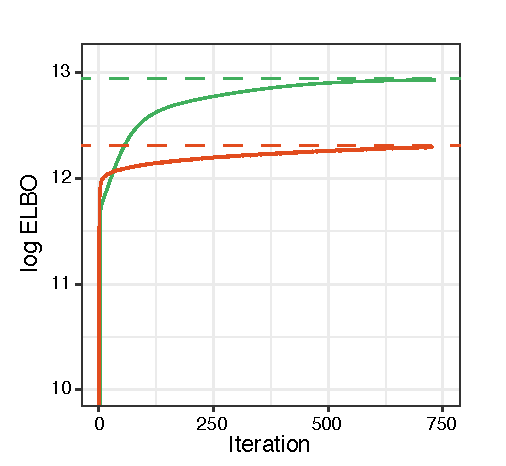
\includegraphics[width=0.5\textwidth]{elbo_convergence}
	\caption{XX}
	\label{fig:elbo_convergence}
\end{figure}

\subsection{Model selection and consistency across random initilizations} \label{section:robustness}
The optimisation problem in MOFA is not convex and the algorithm is not guaranteed to find the optimal solution \cite{XX}. Therefore, posterior distributions will vary depending on the initialisation and it becomes mandatory to perform model selection and assess the consistency of the factors across different trials.\\

The strategy we follow here is to train several MOFA models (e.g. 10 trials) under different parameter initialisations, and subsequently select the model with the highest ELBO for downstream analysis. In addition, we evaluate the robustness of the factors by plotting the Pearson correlations between factors across all trials. \Cref{fig:MOFA_robustness}. 

A similar strategy has also been proposed in \cite{Hore2016}.


\begin{figure}[H]
	\centering 	
	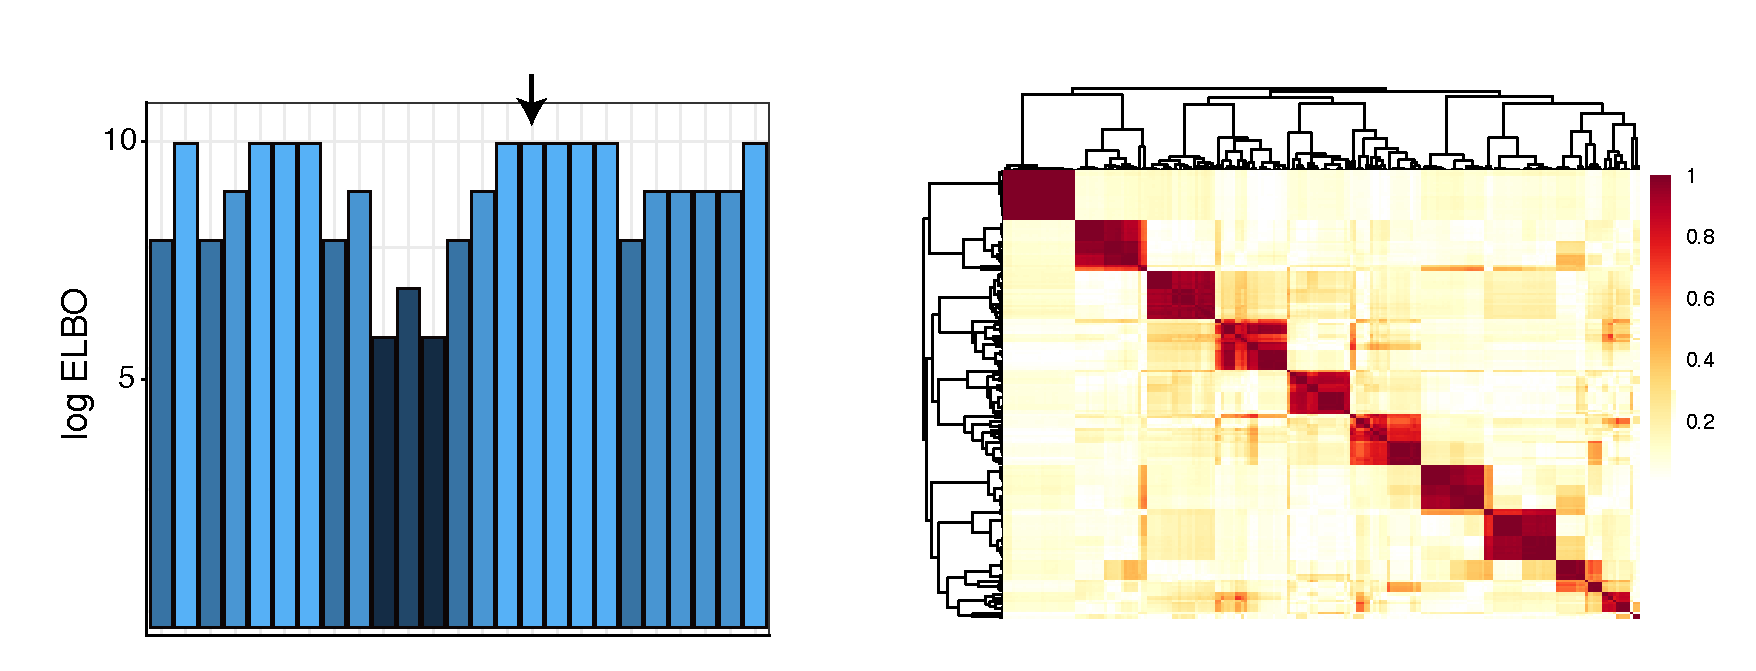
\includegraphics[width=1.0\textwidth]{MOFA_robustness}
	\caption{XX... A block-diagonal matrix ensures good consistency across random initialisations}
	\label{fig:MOFA_robustness}
\end{figure}


% \subsection{Feature Set Enrichment Analysis}

% \subsection{Comparison with previous methods}

%The key difference with the sparse Bayesian factor analysis model in Section XX is that we learn a separate $\alpha_k^m$ and $\theta_k^m$ per factor and view, instead of per factor. This allows the model to take into account that the data is structured into different views.\\



\subsection{Learning the number of factors} \label{section:number_factors}
As described in section X, the use of an ARD prior allows factors to be actively prunned by the model if they explain negligible variation. In the implementation this is controlled by a hyperparameter that defines a threshold on the minimum fraction of variance explained by a factor (across all views).\\
Additionally, because of the non-convexity of the variational inference algorithm, different model instances can potentially yield solutions with different number of active factors (\Cref{fig:mofa_nfactors}). The optimal number of factors need to be selected by the model selection strategy outlined in \Cref{section:robustness}.

\begin{figure}[H]
	\centering 	
	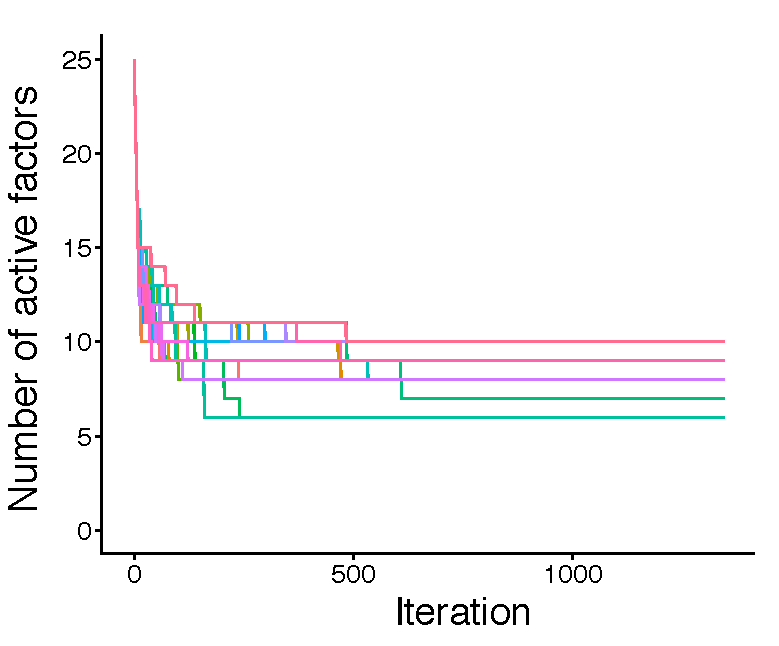
\includegraphics[width=0.5\textwidth]{MOFA_nfactors}
	\caption{XX}
	\label{fig:MOFA_nfactors}
\end{figure}



\subsection{Application to single-cell multi-omics} \label{section:mofa_scmt}

The emergence of single-cell multi-modal techniques has created open opportunities the development of novel computational techniques that integrate data sets across multiple modalities \cite{XX}. Here, we investigated the potential of MOFA to unravel the heterogeneity in one of the earliest single-cell multi-omics data sets \cite{Angermuelller2016}.\\
The data set consists on 87 embryonic stem cells (ESCs) where RNA expression and DNA methylation were simultaneously profiled using single-cell Methylation and Transcriptome sequencing (scM\&T-seq).
Two populations of ESCs were profiled: the first one contains 16 cells grown in 2i media, which induces a native pluripotency state with genome-wide DNA hypomethylation \cite{XX}. the second population contains 71 cells grown in serum media, which triggers a primed pluripotency state poised for differentiation \cite{XX}.\\

The RNA expression data was processed using standard pipelines \cite{Lun2016} to obtain log normalised counts, followed by a selection of the top 5,000 most overdispersed genes \cite{XX}.\\
The DNA methylation data was processed as described in section XXX. Briefly, for each CpG site, we calculated a binary methylation rate from the ratio of methylated read counts to total read counts. Next, CpG sites were classified by overlapping with genomic contexts, namely promoters, CpG islands and enhancers (defined by the presence of distal H3K27ac marks). Finally, for each annotation we selected the top 5,000 most variable CpG sites with a minimum coverage of 10\% across cells.\\
Each of the resulting matrices was input as a separate view to MOFA.\\

In this data set, MOFA learnt 3 factors (minimum explained variance of 2\%). Factor 1 captured the transition from naive to primed pluripotent states, which MOFA links to widespread coordinated changes between DNA methylation and RNA expression. Inspection of the gene loadings for Factor 1 pinpoints important pluripotency markers including  Rex1/Zpf42 or Essrb \cite{XX}. As previously described both in vitro (Angermueller et al, 2016) and in vivo (Auclair et al, 2014), the dynamics of DNA methylation are driven by a genome-wide increase in DNA methylation levels \cite{XX}

Factor 2 captured a second axis of differentiation from a primed pluripotency state to a differentiated state (Figure 6b,c).
e to a differentiated state with highest RNA loadings for known differentiation markers such as keratins and annexins

% Interestingly, the combination of Factors 1 and 2 captured the entire differentiation trajectory from naive pluripotent cells via primed pluripotent cells to differentiated cells, (Figure 6b), illustrating the importance of learning continuous latent factors rather than discrete sample assignments as done by popular methods such as SNF [47] or iCluster [31,

 %Finally, Factor 3 captured the cellular detection rate, a known tech- nical covariate associated with cell quality and mRNA content (Finak et al, 2015; Appendix Fig S22).

%Jointly, Factors 1 and 2 captured the entire differentiation trajec- tory from naive pluripotent cells via primed pluripotent cells to dif- ferentiated cells (Fig 5E), illustrating the importance of learning continuous latent factors rather than discrete sample assignments. Multi-omics clustering algorithms such as SNF (Wang et al, 2014) or iCluster (Shen et al, 2009; Mo et al, 2013) were only capable of distinguishing cellular subpopulations, but not of recovering contin- uous processes such as cell differentiation (Appendix Fig S23).

\begin{figure}[H]
	\centering 	
	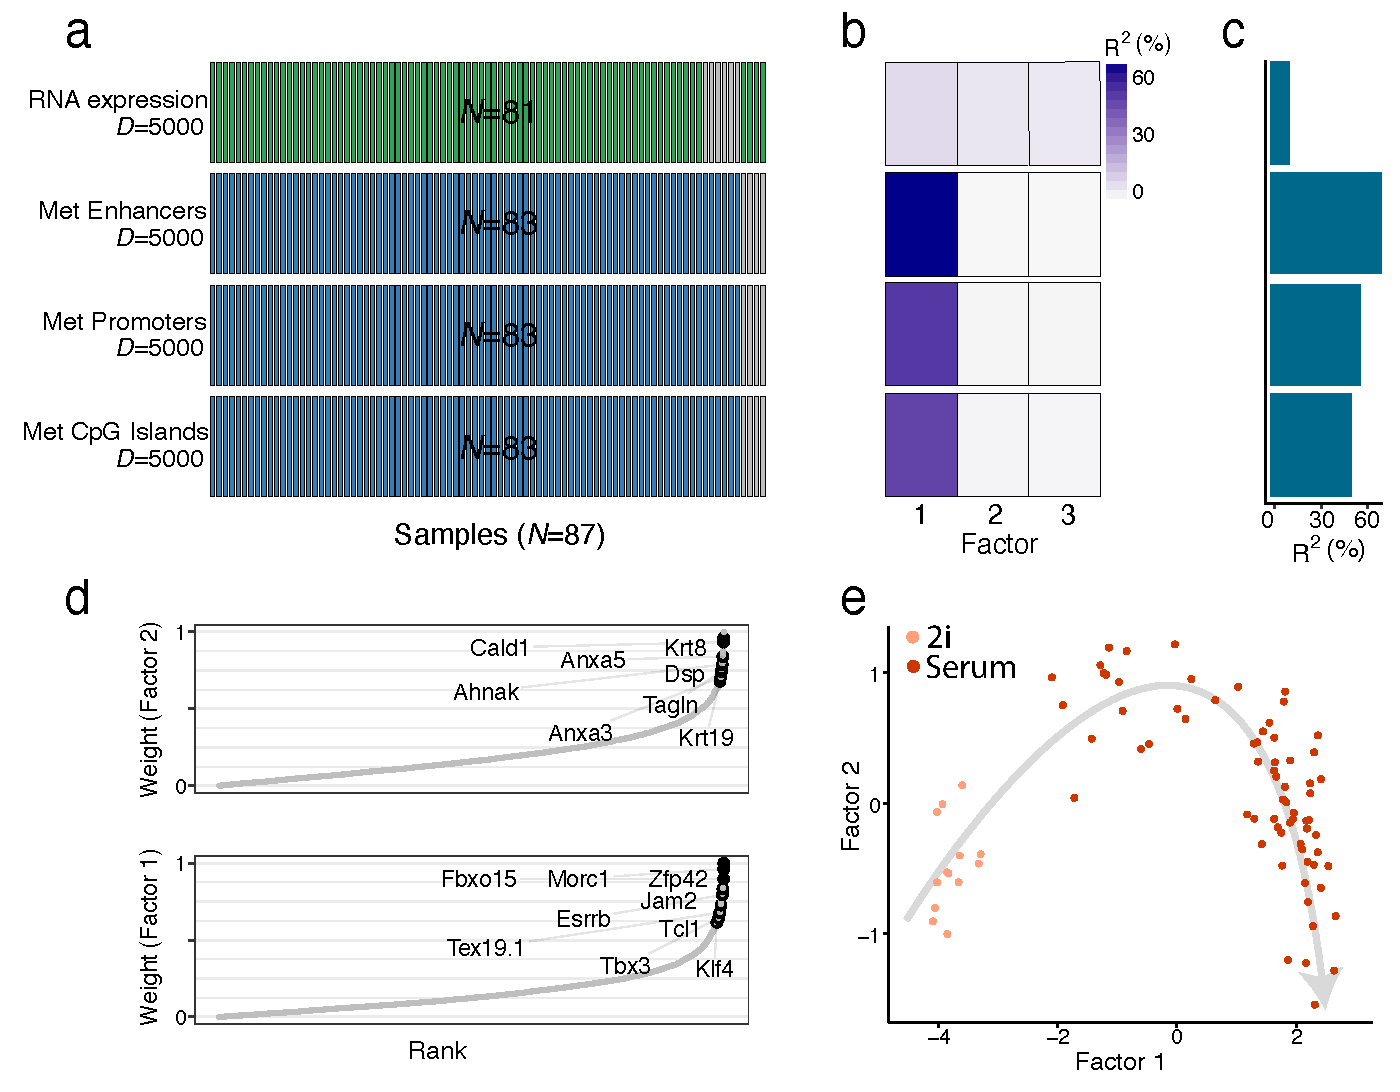
\includegraphics[width=1.0\textwidth]{MOFA_scMT}
	\caption{XX}
	\label{fig:MOFA_scMT}
\end{figure}

% Conclusion: MOFA reveals coordinated changes between the transcriptome and the epigenome along a differentiation trajectory

\subsection{Open perspectives}
% We developed Multi-Omics Factor Analysis (MOFA), an unsupervised method for decomposing the sources of heterogeneity in multi-omics data sets. We illustrated its potential using two data sets with high- dimensional and incomplete multi-omics profiles.
% Although we have addressed important challenges for multi-omics applications, MOFA is not free of limitations. The model is linear, which means that it can miss strongly non-linear relationships between features within and across views. Non-linear extensions of MOFA may address this, although as with any models in high-dimensional spaces, there will be trade-offs between model complexity, computational efficiency and interpretability [14]. Also, a related area of work is to incorporate prior information on the relationships between individual features [6]. Finally, while here we use approximate Bayesian inference and focus attention on the resulting point estimates of inferred factors, future extensions could attempt a more comprehensive Bayesian treatment that propagates evidence strength and estimation uncertainties for diagnostics and downstream analyses [46].

% Although we have addressed important challenges for multi- omics applications, MOFA is not free of limitations. The model is linear, which means that it can miss strongly non-linear relation- ships between features within and across assays (Buettner & Theis, 2012). Non-linear extensions of MOFA may address this, although, as with any models in high-dimensional spaces, there will be trade- offs between model complexity, computational efficiency and inter- pretability (preprint: Damianou et al, 2016). A related area of work is to incorporate prior information on the relationships between individual features. For example, future extensions could make use of pathway databases within each omic type (Buettner et al, 2017) or priors that reflect relationships given by the “dogma of molecular biology”. In addition, new likelihoods and noise models could expand the value of MOFA in data sets with specific statistical prop- erties that hamper the application of traditional statistical methods, including zero-inflated data (i.e. scRNA-Seq; Pierson & Yau, 2015) or binomial distributed data (i.e. splicing events; Huang & Sangui- netti, 2017). Finally, while here we focus our attention on the point estimates of inferred factors, future extensions could attempt a more comprehensive Bayesian treatment that propagates evidence strength and estimation uncertainties to diagnostics and down- stream analyses.